\documentclass{beamer}
\usepackage{amsmath,amssymb,amsfonts,mathrsfs,accents}
\usepackage{array}
\usepackage{graphicx}
\usepackage{caption}
\usepackage{subcaption}
\usepackage[utf8]{inputenc}
%\usetheme{Madrid}
\usecolortheme{default}
\usepackage{blindtext}
\usepackage{hyperref}
\usepackage{multirow}
\usepackage{appendixnumberbeamer}
\setbeamertemplate{caption}[numbered]
\setbeamertemplate{page number in head/foot}[appendixframenumber]
\usepackage{listings}
\usepackage[authoryear]{natbib}
\bibliographystyle{plainnat} 
\renewcommand{\lstlistingname}{Model}
\lstset{frame=none, framexleftmargin=4pt, framexrightmargin=4pt, backgroundcolor=\color{code_bg}, basicstyle=\footnotesize\ttfamily, tabsize=2}

%For different theme%%%%%%%%%%%%%%%%%
\usetheme[progressbar=frametitle]{metropolis}
\usepackage{appendixnumberbeamer}

\usepackage{booktabs}
\usepackage[scale=2]{ccicons}

\usepackage{pgfplots}
\usepgfplotslibrary{dateplot}

\usepackage{xspace}
\newcommand{\themename}{\textbf{\textsc{metropolis}}\xspace}
%%%%%%%%%%%%%%%%%%%%%%%%%%%%%%%%


%-----------------------------------------------------------------------------------%

\begin{document}
\title{Power sector transition dynamics}
\author{Maija Kaartinen and Alireza Azampour}
\date{\today}
\maketitle
	
%----------------------------------------------------------------------------------

\begin{frame}{Review of changes}
\small
\begin{itemize}
\item Since annual efficiency data seemed very volatile, we constructed a new efficiency measure from hourly data, controlling for changes in capacity utilization.
\item The efficiency measure is now the plant fixed effect from these regressions. Update is an efficiency increase above a threshold, such that this doesn't completely recoil in the next period. 
\item The main regression results look similar to before.
\item When plotting, efficiency looks a bit less volatile.
\item We also tried using technological dummy variables and prime mover changes as proxy for technological updates. 
\item The efficiency changes are correlated with capacity increases, less so with technology dummies.
\item Efficiency distributions look more spread out than before if anything.

\end{itemize}
\end{frame}
%%%%%%%%%%%%%%%
\begin{frame}{Some time paths}


\begin{table}
\centering
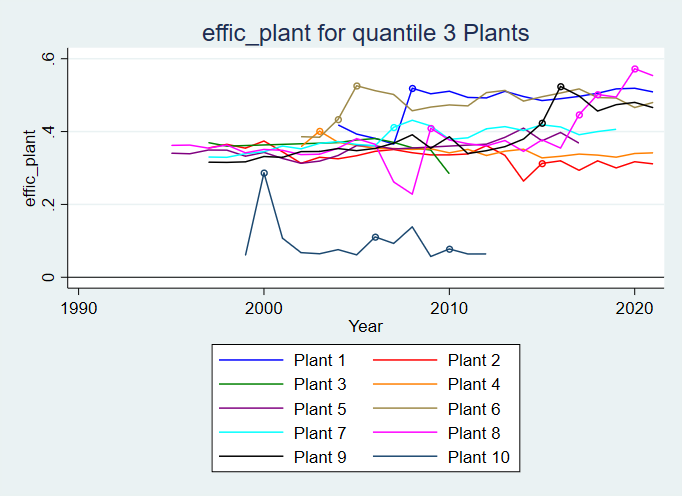
\includegraphics[scale=0.35]{effic_plant_quantile3_allvals.png}
\end{table}
\footnotesize{Note: Efficiency update at least 10 \% increase such that efficiency in the following period remains higher than before update.}

\end{frame}
    
%%%%%%%%%%%%%%%
\begin{frame}{Efficiency after previous update and update likelihood}


\begin{table}
\centering
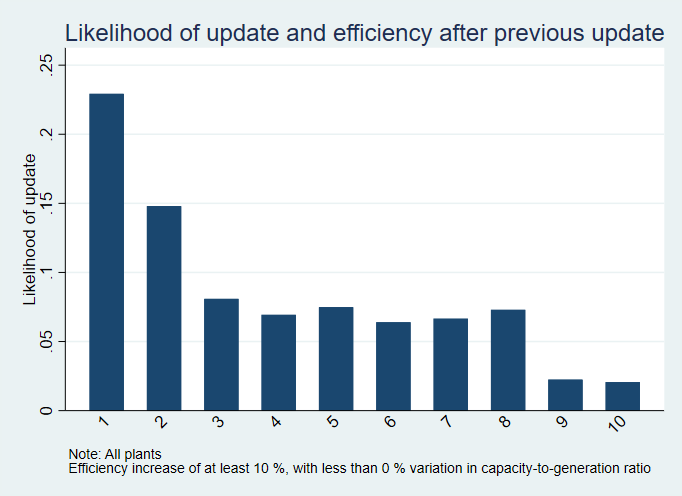
\includegraphics[scale=0.4]{hist_effic_updatedummy_all.png}
\end{table}
\footnotesize{Note: Efficiency update at least 10 \% increase such that efficiency in the following period remains higher than before update.}
\end{frame}
    
%%%%%%%%%%%%%%%
\begin{frame}{Update likelihood, efficiency and age}


\begin{table}
\centering
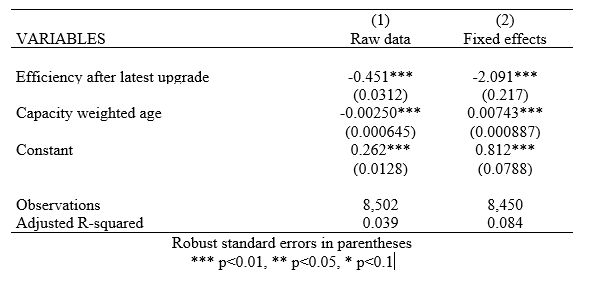
\includegraphics[scale=0.6]{Main regression_10_all.PNG}
\end{table}
\footnotesize{Note: Efficiency update at least 10 \% increase such that efficiency in the following period remains higher than before update.}
\end{frame}
    
%%%%%%%%%%%%%%%
\begin{frame}{Update likelihood, efficiency and age, cohort effects}


\begin{table}
\centering
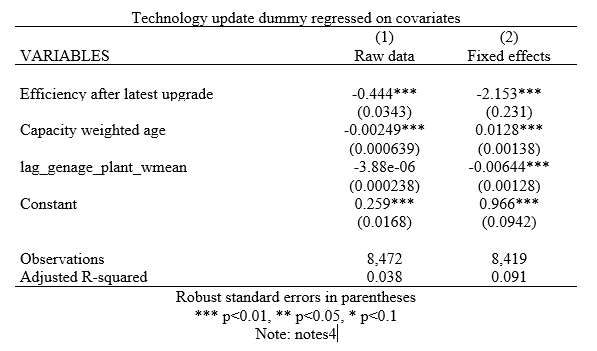
\includegraphics[scale=0.6]{Main regression_10_all_genage.PNG}
\end{table}
\footnotesize{Note: Efficiency update at least 10 \% increase such that efficiency in the following period remains higher than before update.}
\end{frame}
    
%%%%%%%%%%%%%%%
\begin{frame}{Efficiency and long-term quality component}


\begin{table}
\centering
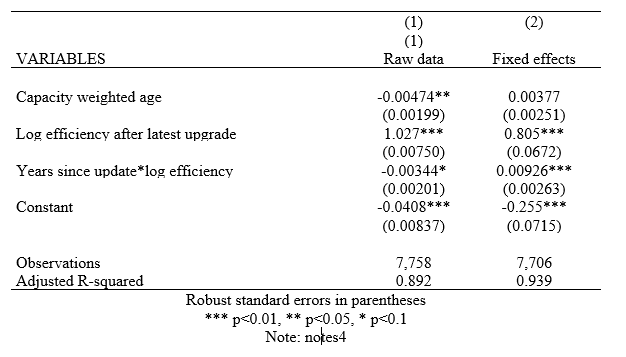
\includegraphics[scale=0.6]{logeffic_capageinteract_10_all.PNG}
\end{table}

\end{frame}
    
%%%%%%%%%%%%%%%
\begin{frame}{Calibration: efficiency distribution, all}

\begin{table}
\centering
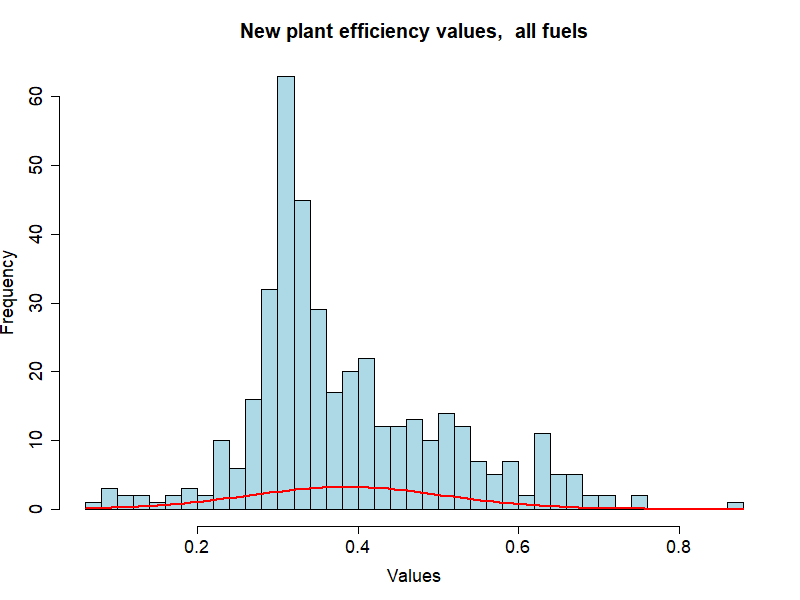
\includegraphics[scale=0.3]{efficdist_all_norm_hist.png}
\end{table}



\end{frame}

%%%%%%%%%%%%%%%
\begin{frame}{Calibration: efficiency distribution, old technology}

\begin{table}
\centering
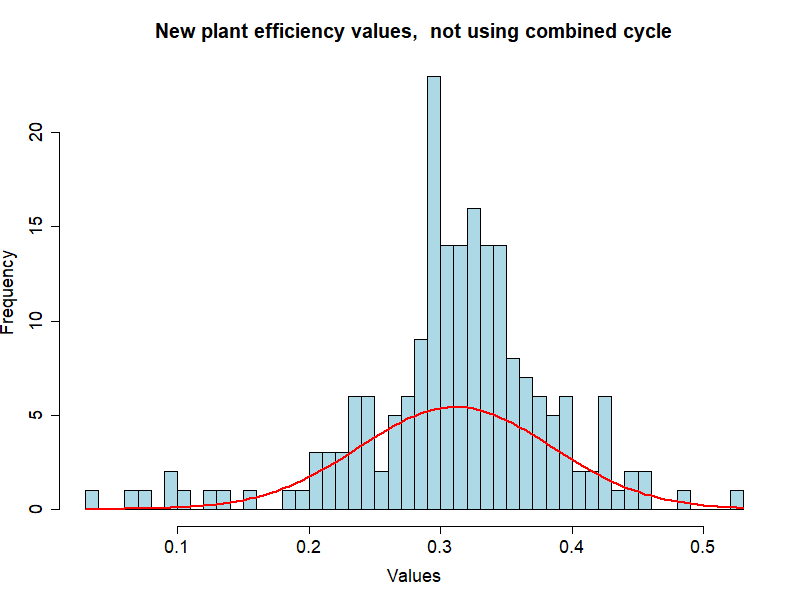
\includegraphics[scale=0.3]{efficdist_noCC_norm_hist.png}
\end{table}



\end{frame}

%%%%%%%%%%%%%%%

\begin{frame}{Calibration: efficiency distribution, new technology}

\begin{table}
\centering
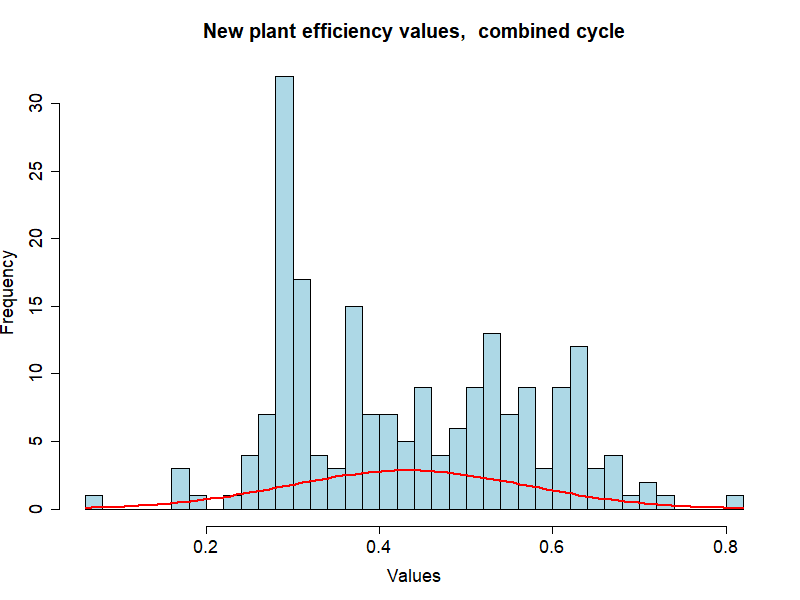
\includegraphics[scale=0.3]{efficdist_CC_norm_hist.png}
\end{table}



\end{frame}

%%%%%%%%%%%%%%%


\begin{frame}{Correlations with capacity, tech variable dummies}


\begin{table}
\centering
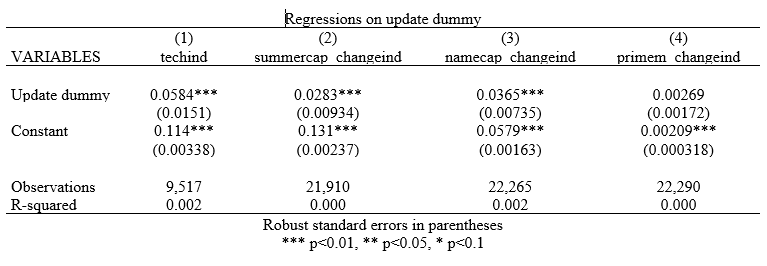
\includegraphics[scale=0.55]{capacity_efficreg_dummies_10.PNG}
\end{table}
\footnotesize{Note: Efficiency update at least 10 \% increase such that efficiency in the following period remains higher than before update.}

\end{frame}
    
%%%%%%%%%%%%%%%
\begin{frame}{Correlations with capacity}


\begin{table}
\centering
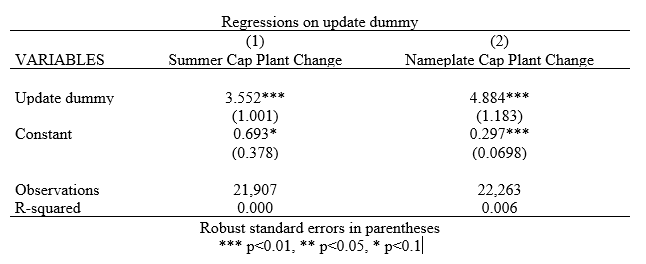
\includegraphics[scale=0.55]{capacity_efficreg_continuous_10.PNG}
\end{table}
\footnotesize{Note: Efficiency update at least 10 \% increase such that efficiency in the following period remains higher than before update.}
\end{frame}
    
%%%%%%%%%%%%%%%
\begin{frame}{Tabulations}


\begin{table}
\centering
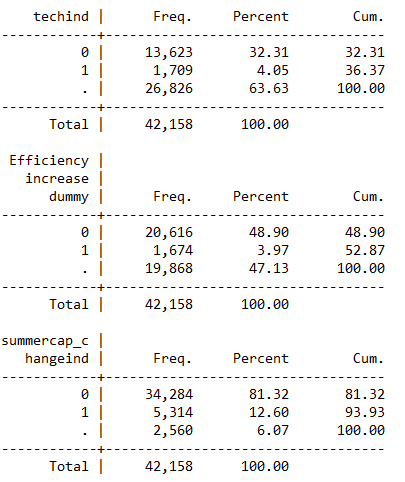
\includegraphics[scale=0.5]{tabulations_10.PNG}
\end{table}
\footnotesize{Note: Efficiency update at least 10 \% increase such that efficiency in the following period remains higher than before update.}
\end{frame}
    
%%%%%%%%%%%%%%%

\begin{frame}{Tech variable mean by update dummy}


\begin{table}
\centering
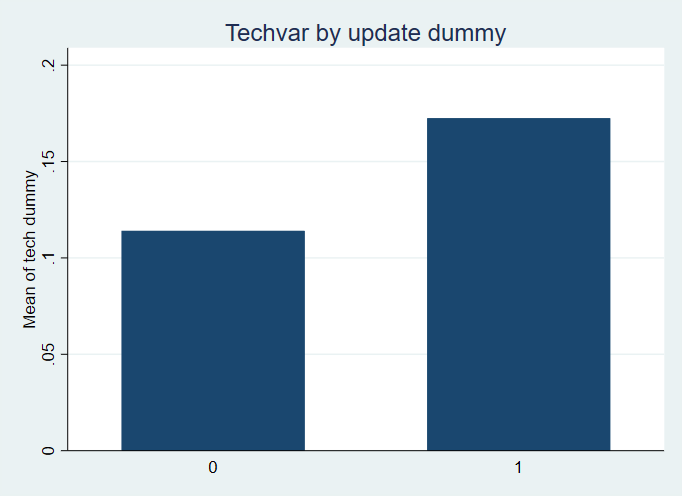
\includegraphics[scale=0.35]{techind_by_update.png}
\end{table}
\footnotesize{Note: Efficiency update at least 10 \% increase such that efficiency in the following period remains higher than before update.}
\end{frame}
    
%%%%%%%%%%%%%%%
\begin{frame}{Capacity change mean by update dummy}


\begin{table}
\centering
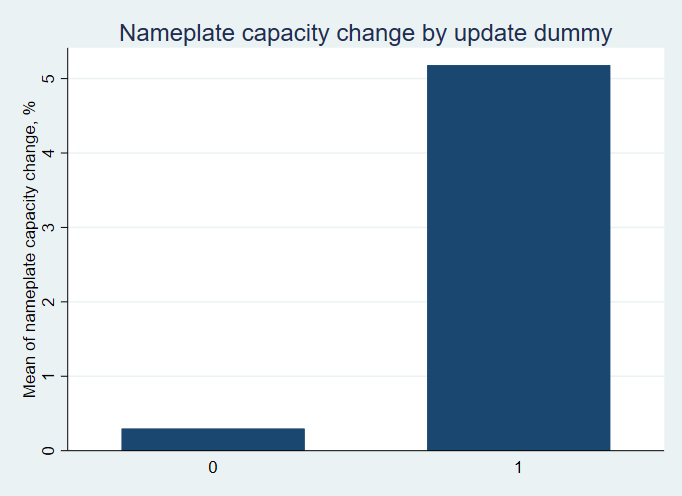
\includegraphics[scale=0.35]{nameplatecapchange_by_update.png}
\end{table}
\footnotesize{Note: Efficiency update at least 10 \% increase such that efficiency in the following period remains higher than before update.}
\end{frame}
    
%%%%%%%%%%%%%%%
\begin{frame}{Model: household side}

\begin{itemize}
    \item Adding a consumer side to get closer to welfare effects.
    \item Households have Cobb-Douglas preferences over electricity and other goods.
    \item They earn a constant exogenous income and electricity firm profits and pay/receive taxes/transfers.
    \item Household utility is impacted by climate damages.
\end{itemize}
\footnotesize\begin{align*}
    \mathcal{U}&=E^\alpha Y^{1-\alpha}-\phi S\\
    I&=I_{exo}  - \tau_h \\
    V_j &= \int\big\{ p_Ea_{i,0} e_i^\alpha -p_e e_i+E[v(a_{i,0},1)] \big\} dD(a_{i,0})-c_{e} + su_j = 0\\
    v(a_{i},t) &= \max_{e_i,ad=\{0,1\}} p_E\frac{a_{i}^{1+\gamma t}}{(1+g_a)^t} e_i^\alpha -(p_e + \tau_e) e_i-c_f\\ 
    &+\beta \big(\mathbf{1}_{\{ad =0\}} \mathbb{E}[v(a_{i},t+1)]  + \mathbf{1}_{\{ad =1\}}[ \mathbb{E}[v(a_{i}',t-\tau)]-c_a]\big)\\
    &\int_i \tau_e e_i di - \int_i su_idi +\tau_h = 0
\end{align*}

\end{frame}
    
%%%%%%%%%%%%%%%
\begin{frame}{Model: household side}
\small
\begin{itemize}
    \item To solve for the optimal path of carbon taxes and subsidies, we first solve the planner's problem for a given emission target without considering carbon damages,
    \item Then, if the shape of the policies is the same regardless of target, we solve for the optimal climate target by maximizing household welfare considering both carbon damages and the abatement costs on optimal path for a given target.
    \item We solve this separately for both subsidies, a carbon tax, and a combination of both policies.
\end{itemize}

\end{frame}
    
%%%%%%%%%%%%%%%


\end{document}